\documentclass[]{article}
\usepackage{lmodern}
\usepackage{amssymb,amsmath}
\usepackage{ifxetex,ifluatex}
\usepackage{fixltx2e} % provides \textsubscript
\ifnum 0\ifxetex 1\fi\ifluatex 1\fi=0 % if pdftex
  \usepackage[T1]{fontenc}
  \usepackage[utf8]{inputenc}
\else % if luatex or xelatex
  \ifxetex
    \usepackage{mathspec}
  \else
    \usepackage{fontspec}
  \fi
  \defaultfontfeatures{Ligatures=TeX,Scale=MatchLowercase}
\fi
% use upquote if available, for straight quotes in verbatim environments
\IfFileExists{upquote.sty}{\usepackage{upquote}}{}
% use microtype if available
\IfFileExists{microtype.sty}{%
\usepackage{microtype}
\UseMicrotypeSet[protrusion]{basicmath} % disable protrusion for tt fonts
}{}
\usepackage[margin=1in]{geometry}
\usepackage{hyperref}
\hypersetup{unicode=true,
            pdftitle={Naive Bayes},
            pdfauthor={Jared Salinas},
            pdfborder={0 0 0},
            breaklinks=true}
\urlstyle{same}  % don't use monospace font for urls
\usepackage{color}
\usepackage{fancyvrb}
\newcommand{\VerbBar}{|}
\newcommand{\VERB}{\Verb[commandchars=\\\{\}]}
\DefineVerbatimEnvironment{Highlighting}{Verbatim}{commandchars=\\\{\}}
% Add ',fontsize=\small' for more characters per line
\usepackage{framed}
\definecolor{shadecolor}{RGB}{248,248,248}
\newenvironment{Shaded}{\begin{snugshade}}{\end{snugshade}}
\newcommand{\KeywordTok}[1]{\textcolor[rgb]{0.13,0.29,0.53}{\textbf{#1}}}
\newcommand{\DataTypeTok}[1]{\textcolor[rgb]{0.13,0.29,0.53}{#1}}
\newcommand{\DecValTok}[1]{\textcolor[rgb]{0.00,0.00,0.81}{#1}}
\newcommand{\BaseNTok}[1]{\textcolor[rgb]{0.00,0.00,0.81}{#1}}
\newcommand{\FloatTok}[1]{\textcolor[rgb]{0.00,0.00,0.81}{#1}}
\newcommand{\ConstantTok}[1]{\textcolor[rgb]{0.00,0.00,0.00}{#1}}
\newcommand{\CharTok}[1]{\textcolor[rgb]{0.31,0.60,0.02}{#1}}
\newcommand{\SpecialCharTok}[1]{\textcolor[rgb]{0.00,0.00,0.00}{#1}}
\newcommand{\StringTok}[1]{\textcolor[rgb]{0.31,0.60,0.02}{#1}}
\newcommand{\VerbatimStringTok}[1]{\textcolor[rgb]{0.31,0.60,0.02}{#1}}
\newcommand{\SpecialStringTok}[1]{\textcolor[rgb]{0.31,0.60,0.02}{#1}}
\newcommand{\ImportTok}[1]{#1}
\newcommand{\CommentTok}[1]{\textcolor[rgb]{0.56,0.35,0.01}{\textit{#1}}}
\newcommand{\DocumentationTok}[1]{\textcolor[rgb]{0.56,0.35,0.01}{\textbf{\textit{#1}}}}
\newcommand{\AnnotationTok}[1]{\textcolor[rgb]{0.56,0.35,0.01}{\textbf{\textit{#1}}}}
\newcommand{\CommentVarTok}[1]{\textcolor[rgb]{0.56,0.35,0.01}{\textbf{\textit{#1}}}}
\newcommand{\OtherTok}[1]{\textcolor[rgb]{0.56,0.35,0.01}{#1}}
\newcommand{\FunctionTok}[1]{\textcolor[rgb]{0.00,0.00,0.00}{#1}}
\newcommand{\VariableTok}[1]{\textcolor[rgb]{0.00,0.00,0.00}{#1}}
\newcommand{\ControlFlowTok}[1]{\textcolor[rgb]{0.13,0.29,0.53}{\textbf{#1}}}
\newcommand{\OperatorTok}[1]{\textcolor[rgb]{0.81,0.36,0.00}{\textbf{#1}}}
\newcommand{\BuiltInTok}[1]{#1}
\newcommand{\ExtensionTok}[1]{#1}
\newcommand{\PreprocessorTok}[1]{\textcolor[rgb]{0.56,0.35,0.01}{\textit{#1}}}
\newcommand{\AttributeTok}[1]{\textcolor[rgb]{0.77,0.63,0.00}{#1}}
\newcommand{\RegionMarkerTok}[1]{#1}
\newcommand{\InformationTok}[1]{\textcolor[rgb]{0.56,0.35,0.01}{\textbf{\textit{#1}}}}
\newcommand{\WarningTok}[1]{\textcolor[rgb]{0.56,0.35,0.01}{\textbf{\textit{#1}}}}
\newcommand{\AlertTok}[1]{\textcolor[rgb]{0.94,0.16,0.16}{#1}}
\newcommand{\ErrorTok}[1]{\textcolor[rgb]{0.64,0.00,0.00}{\textbf{#1}}}
\newcommand{\NormalTok}[1]{#1}
\usepackage{graphicx,grffile}
\makeatletter
\def\maxwidth{\ifdim\Gin@nat@width>\linewidth\linewidth\else\Gin@nat@width\fi}
\def\maxheight{\ifdim\Gin@nat@height>\textheight\textheight\else\Gin@nat@height\fi}
\makeatother
% Scale images if necessary, so that they will not overflow the page
% margins by default, and it is still possible to overwrite the defaults
% using explicit options in \includegraphics[width, height, ...]{}
\setkeys{Gin}{width=\maxwidth,height=\maxheight,keepaspectratio}
\IfFileExists{parskip.sty}{%
\usepackage{parskip}
}{% else
\setlength{\parindent}{0pt}
\setlength{\parskip}{6pt plus 2pt minus 1pt}
}
\setlength{\emergencystretch}{3em}  % prevent overfull lines
\providecommand{\tightlist}{%
  \setlength{\itemsep}{0pt}\setlength{\parskip}{0pt}}
\setcounter{secnumdepth}{0}
% Redefines (sub)paragraphs to behave more like sections
\ifx\paragraph\undefined\else
\let\oldparagraph\paragraph
\renewcommand{\paragraph}[1]{\oldparagraph{#1}\mbox{}}
\fi
\ifx\subparagraph\undefined\else
\let\oldsubparagraph\subparagraph
\renewcommand{\subparagraph}[1]{\oldsubparagraph{#1}\mbox{}}
\fi

%%% Use protect on footnotes to avoid problems with footnotes in titles
\let\rmarkdownfootnote\footnote%
\def\footnote{\protect\rmarkdownfootnote}

%%% Change title format to be more compact
\usepackage{titling}

% Create subtitle command for use in maketitle
\newcommand{\subtitle}[1]{
  \posttitle{
    \begin{center}\large#1\end{center}
    }
}

\setlength{\droptitle}{-2em}

  \title{Naive Bayes}
    \pretitle{\vspace{\droptitle}\centering\huge}
  \posttitle{\par}
    \author{Jared Salinas}
    \preauthor{\centering\large\emph}
  \postauthor{\par}
      \predate{\centering\large\emph}
  \postdate{\par}
    \date{21/1/2019}


\begin{document}
\maketitle

\subsubsection{Leyendo la información}\label{leyendo-la-informacion}

\begin{Shaded}
\begin{Highlighting}[]
\NormalTok{sms_raw<-}\KeywordTok{read.csv}\NormalTok{(}\StringTok{"data/sms_spam.csv"}\NormalTok{,}\DataTypeTok{stringsAsFactors =} \OtherTok{FALSE}\NormalTok{)}
\end{Highlighting}
\end{Shaded}

Vemos información del dataset

\begin{Shaded}
\begin{Highlighting}[]
\KeywordTok{str}\NormalTok{(sms_raw)}
\end{Highlighting}
\end{Shaded}

\begin{verbatim}
## 'data.frame':    5574 obs. of  2 variables:
##  $ type: chr  "ham" "ham" "spam" "ham" ...
##  $ text: chr  "Go until jurong point, crazy.. Available only in bugis n great world la e buffet... Cine there got amore wat..." "Ok lar... Joking wif u oni..." "Free entry in 2 a wkly comp to win FA Cup final tkts 21st May 2005. Text FA to 87121 to receive entry question("| __truncated__ "U dun say so early hor... U c already then say..." ...
\end{verbatim}

La información son el texto, y una clasificación (spam o ham)

\subsection{Vemos información estadistica del caso de
estudio}\label{vemos-informacion-estadistica-del-caso-de-estudio}

\begin{Shaded}
\begin{Highlighting}[]
\KeywordTok{summary}\NormalTok{(sms_raw)}
\end{Highlighting}
\end{Shaded}

\begin{verbatim}
##      type               text          
##  Length:5574        Length:5574       
##  Class :character   Class :character  
##  Mode  :character   Mode  :character
\end{verbatim}

Número de spam y ham

\begin{Shaded}
\begin{Highlighting}[]
\KeywordTok{table}\NormalTok{(sms_raw}\OperatorTok{$}\NormalTok{type)}
\end{Highlighting}
\end{Shaded}

\begin{verbatim}
## 
##  ham spam 
## 4827  747
\end{verbatim}

Hay más información sobre ham que de spam

\subsection{Procesamiento de los
datos}\label{procesamiento-de-los-datos}

Como es un conjunto de texto, tenemos que hacer una limpieza de los
datos, quitar información irrelevante para el clasificador, tener en
cuenta que es importante saber que los mensajes que contienen spam, te
regalan algo, o te dan algo muy dificil de obtener. Es por eso que usan
mucho la palabra ``free''

\begin{Shaded}
\begin{Highlighting}[]
\CommentTok{#importamos librería necesaria}
\KeywordTok{library}\NormalTok{(tm)}
\end{Highlighting}
\end{Shaded}

\begin{verbatim}
## Loading required package: NLP
\end{verbatim}

\begin{Shaded}
\begin{Highlighting}[]
\NormalTok{sms_corpus<-}\KeywordTok{VCorpus}\NormalTok{(}\KeywordTok{VectorSource}\NormalTok{(sms_raw}\OperatorTok{$}\NormalTok{text))}

\KeywordTok{print}\NormalTok{(sms_corpus)}
\end{Highlighting}
\end{Shaded}

\begin{verbatim}
## <<VCorpus>>
## Metadata:  corpus specific: 0, document level (indexed): 0
## Content:  documents: 5574
\end{verbatim}

Hacemos elementos de tipo documentos.

visualizamos los datos de los documentos.

\begin{Shaded}
\begin{Highlighting}[]
\CommentTok{# visualizar los datos del corpus}
\KeywordTok{inspect}\NormalTok{(sms_corpus[}\DecValTok{1}\OperatorTok{:}\DecValTok{2}\NormalTok{])}
\end{Highlighting}
\end{Shaded}

\begin{verbatim}
## <<VCorpus>>
## Metadata:  corpus specific: 0, document level (indexed): 0
## Content:  documents: 2
## 
## [[1]]
## <<PlainTextDocument>>
## Metadata:  7
## Content:  chars: 111
## 
## [[2]]
## <<PlainTextDocument>>
## Metadata:  7
## Content:  chars: 29
\end{verbatim}

\begin{Shaded}
\begin{Highlighting}[]
\KeywordTok{as.character}\NormalTok{(sms_corpus[[}\DecValTok{1}\NormalTok{]])}
\end{Highlighting}
\end{Shaded}

\begin{verbatim}
## [1] "Go until jurong point, crazy.. Available only in bugis n great world la e buffet... Cine there got amore wat..."
\end{verbatim}

La función lappy nos deja poder más de dos documentos, ya que afecta al
conjunto

\begin{Shaded}
\begin{Highlighting}[]
\KeywordTok{lapply}\NormalTok{(sms_corpus[}\DecValTok{1}\OperatorTok{:}\DecValTok{2}\NormalTok{], as.character)}
\end{Highlighting}
\end{Shaded}

\begin{verbatim}
## $`1`
## [1] "Go until jurong point, crazy.. Available only in bugis n great world la e buffet... Cine there got amore wat..."
## 
## $`2`
## [1] "Ok lar... Joking wif u oni..."
\end{verbatim}

Primero tenemos que hacer que nuestras cadenas de texto esten todas en
minusculas

\begin{Shaded}
\begin{Highlighting}[]
\NormalTok{sms_corpus_clean<-}\KeywordTok{tm_map}\NormalTok{(sms_corpus, }\KeywordTok{content_transformer}\NormalTok{(tolower))}

\KeywordTok{as.character}\NormalTok{(sms_corpus[[}\DecValTok{1}\NormalTok{]])}
\end{Highlighting}
\end{Shaded}

\begin{verbatim}
## [1] "Go until jurong point, crazy.. Available only in bugis n great world la e buffet... Cine there got amore wat..."
\end{verbatim}

\begin{Shaded}
\begin{Highlighting}[]
\KeywordTok{as.character}\NormalTok{(sms_corpus_clean[[}\DecValTok{1}\NormalTok{]])}
\end{Highlighting}
\end{Shaded}

\begin{verbatim}
## [1] "go until jurong point, crazy.. available only in bugis n great world la e buffet... cine there got amore wat..."
\end{verbatim}

Removemos Números de nuestros textos

\begin{Shaded}
\begin{Highlighting}[]
\NormalTok{sms_corpus_clean<-}\KeywordTok{tm_map}\NormalTok{(sms_corpus_clean,removeNumbers)}
\end{Highlighting}
\end{Shaded}

También información irrelevante, en nuestro caso, son los nexos,
uniones. Para eso usamos la función stopwords y tambien puntuaciones con
con removePunctuation

\begin{Shaded}
\begin{Highlighting}[]
\NormalTok{sms_corpus_clean<-}\KeywordTok{tm_map}\NormalTok{(sms_corpus_clean,removeWords,}\KeywordTok{stopwords}\NormalTok{())}
\NormalTok{sms_corpus_clean<-}\KeywordTok{tm_map}\NormalTok{(sms_corpus_clean,removePunctuation)}
\KeywordTok{as.character}\NormalTok{(sms_corpus_clean[[}\DecValTok{1}\NormalTok{]])}
\end{Highlighting}
\end{Shaded}

\begin{verbatim}
## [1] "go  jurong point crazy available   bugis n great world la e buffet cine  got amore wat"
\end{verbatim}

\begin{Shaded}
\begin{Highlighting}[]
\KeywordTok{library}\NormalTok{(SnowballC)}
\end{Highlighting}
\end{Shaded}

WordStem nos saca la radical de las palabras

\begin{Shaded}
\begin{Highlighting}[]
\KeywordTok{wordStem}\NormalTok{(}\KeywordTok{c}\NormalTok{(}\StringTok{"learn"}\NormalTok{, }\StringTok{"learned"}\NormalTok{, }\StringTok{"learning"}\NormalTok{,}\StringTok{"learns"}\NormalTok{))}
\end{Highlighting}
\end{Shaded}

\begin{verbatim}
## [1] "learn" "learn" "learn" "learn"
\end{verbatim}

\begin{Shaded}
\begin{Highlighting}[]
\KeywordTok{wordStem}\NormalTok{(}\KeywordTok{c}\NormalTok{(}\StringTok{"videogamer"}\NormalTok{,}\StringTok{"gamer"}\NormalTok{,}\StringTok{"gaming"}\NormalTok{,}\StringTok{"gamer"}\NormalTok{))}
\end{Highlighting}
\end{Shaded}

\begin{verbatim}
## [1] "videogam" "gamer"    "game"     "gamer"
\end{verbatim}

\begin{Shaded}
\begin{Highlighting}[]
\NormalTok{sms_corpus_clean<-}\KeywordTok{tm_map}\NormalTok{(sms_corpus_clean, stemDocument)}
\KeywordTok{as.character}\NormalTok{(sms_corpus_clean[[}\DecValTok{1}\NormalTok{]])}
\end{Highlighting}
\end{Shaded}

\begin{verbatim}
## [1] "go jurong point crazi avail bugi n great world la e buffet cine got amor wat"
\end{verbatim}

Removemos espacios vacios

\begin{Shaded}
\begin{Highlighting}[]
\NormalTok{sms_corpus_clean<-}\KeywordTok{tm_map}\NormalTok{(sms_corpus_clean, stripWhitespace)}

\CommentTok{#print(as.character(sms_corpus[1:3]))}
\CommentTok{#as.character(sms_corpus[1:3])}
\KeywordTok{print}\NormalTok{(}\KeywordTok{as.character}\NormalTok{(sms_corpus_clean[}\DecValTok{1}\OperatorTok{:}\DecValTok{3}\NormalTok{]))}
\end{Highlighting}
\end{Shaded}

\begin{verbatim}
## [1] "list(list(content = \"go jurong point crazi avail bugi n great world la e buffet cine got amor wat\", meta = list(author = character(0), datetimestamp = list(sec = 7.80083203315735, min = 46, hour = 6, mday = 22, mon = 0, year = 119, wday = 2, yday = 21, isdst = 0), description = character(0), heading = character(0), id = \"1\", language = \"en\", origin = character(0))), list(content = \"ok lar joke wif u oni\", meta = list(author = character(0), datetimestamp = list(sec = 7.80124592781067, min = 46, hour = 6, \n    mday = 22, mon = 0, year = 119, wday = 2, yday = 21, isdst = 0), description = character(0), heading = character(0), id = \"2\", language = \"en\", origin = character(0))), list(content = \"free entri wkli comp win fa cup final tkts st may text fa receiv entri questionstd txt ratetc appli s\", meta = list(author = character(0), datetimestamp = list(sec = 7.80130910873413, min = 46, hour = 6, mday = 22, mon = 0, year = 119, wday = 2, yday = 21, isdst = 0), description = character(0), heading = character(0), \n    id = \"3\", language = \"en\", origin = character(0))))"
## [2] "list()"                                                                                                                                                                                                                                                                                                                                                                                                                                                                                                                                                                                                                                                                                                                                                                                                                                                                                                                                                                                                                                                                                                                                  
## [3] "list()"
\end{verbatim}

\begin{Shaded}
\begin{Highlighting}[]
\KeywordTok{as.character}\NormalTok{(sms_corpus_clean[}\DecValTok{1}\NormalTok{])}
\end{Highlighting}
\end{Shaded}

\begin{verbatim}
## [1] "list(list(content = \"go jurong point crazi avail bugi n great world la e buffet cine got amor wat\", meta = list(author = character(0), datetimestamp = list(sec = 7.80083203315735, min = 46, hour = 6, mday = 22, mon = 0, year = 119, wday = 2, yday = 21, isdst = 0), description = character(0), heading = character(0), id = \"1\", language = \"en\", origin = character(0))))"
## [2] "list()"                                                                                                                                                                                                                                                                                                                                                                                
## [3] "list()"
\end{verbatim}

\subsection{Preparación de los datos}\label{preparacion-de-los-datos}

\begin{Shaded}
\begin{Highlighting}[]
\NormalTok{sms_dtm<-}\KeywordTok{DocumentTermMatrix}\NormalTok{(sms_corpus_clean)}
\end{Highlighting}
\end{Shaded}

Pudimos haber hecho todo lo anterior con la siguiente linea:

\begin{Shaded}
\begin{Highlighting}[]
\NormalTok{sms_dtm2<-}\KeywordTok{DocumentTermMatrix}\NormalTok{(sms_corpus,}
                             \DataTypeTok{control =} \KeywordTok{list}\NormalTok{(}\DataTypeTok{tolower=}\OtherTok{TRUE}\NormalTok{,}
                                            \DataTypeTok{removeNumbers=}\OtherTok{TRUE}\NormalTok{,}
                                            \DataTypeTok{stopwords=}\OtherTok{TRUE}\NormalTok{,}
                                            \DataTypeTok{removePunctuation=}\OtherTok{TRUE}\NormalTok{,}
                                            \DataTypeTok{stemming=}\OtherTok{TRUE}\NormalTok{))}
\end{Highlighting}
\end{Shaded}

\begin{Shaded}
\begin{Highlighting}[]
\NormalTok{sms_dtm}
\end{Highlighting}
\end{Shaded}

\begin{verbatim}
## <<DocumentTermMatrix (documents: 5574, terms: 6592)>>
## Non-/sparse entries: 42608/36701200
## Sparsity           : 100%
## Maximal term length: 40
## Weighting          : term frequency (tf)
\end{verbatim}

\begin{Shaded}
\begin{Highlighting}[]
\NormalTok{sms_dtm2}
\end{Highlighting}
\end{Shaded}

\begin{verbatim}
## <<DocumentTermMatrix (documents: 5574, terms: 6995)>>
## Non-/sparse entries: 43713/38946417
## Sparsity           : 100%
## Maximal term length: 40
## Weighting          : term frequency (tf)
\end{verbatim}

\begin{Shaded}
\begin{Highlighting}[]
\NormalTok{sms_dtm_train<-sms_dtm[}\DecValTok{1}\OperatorTok{:}\DecValTok{4169}\NormalTok{,]}
\NormalTok{sms_dtm_test<-sms_dtm[}\DecValTok{4170}\OperatorTok{:}\DecValTok{5559}\NormalTok{,]}

\NormalTok{sms_train_labels<-sms_raw[}\DecValTok{1}\OperatorTok{:}\DecValTok{4169}\NormalTok{,]}\OperatorTok{$}\NormalTok{type}
\NormalTok{sms_test_labels<-sms_raw[}\DecValTok{4170}\OperatorTok{:}\DecValTok{5559}\NormalTok{,]}\OperatorTok{$}\NormalTok{type}

\KeywordTok{prop.table}\NormalTok{(}\KeywordTok{table}\NormalTok{(sms_train_labels))}
\end{Highlighting}
\end{Shaded}

\begin{verbatim}
## sms_train_labels
##       ham      spam 
## 0.8647158 0.1352842
\end{verbatim}

\begin{Shaded}
\begin{Highlighting}[]
\KeywordTok{prop.table}\NormalTok{(}\KeywordTok{table}\NormalTok{(sms_test_labels))}
\end{Highlighting}
\end{Shaded}

\begin{verbatim}
## sms_test_labels
##       ham      spam 
## 0.8697842 0.1302158
\end{verbatim}

Hacemos los cortes de prueba y entrenamiento y vemos la distribución del
ham y el spam

\subsection{Visualizando la
información}\label{visualizando-la-informacion}

Además hacemos una nube de palabras para identificar las palabras más
sonadas en el documento.

\begin{Shaded}
\begin{Highlighting}[]
\KeywordTok{library}\NormalTok{(wordcloud)}
\end{Highlighting}
\end{Shaded}

\begin{verbatim}
## Loading required package: RColorBrewer
\end{verbatim}

\begin{Shaded}
\begin{Highlighting}[]
\KeywordTok{wordcloud}\NormalTok{(sms_corpus_clean,}\DataTypeTok{min.freq =} \DecValTok{50}\NormalTok{, }\DataTypeTok{random.order =} \OtherTok{FALSE}\NormalTok{)}
\end{Highlighting}
\end{Shaded}

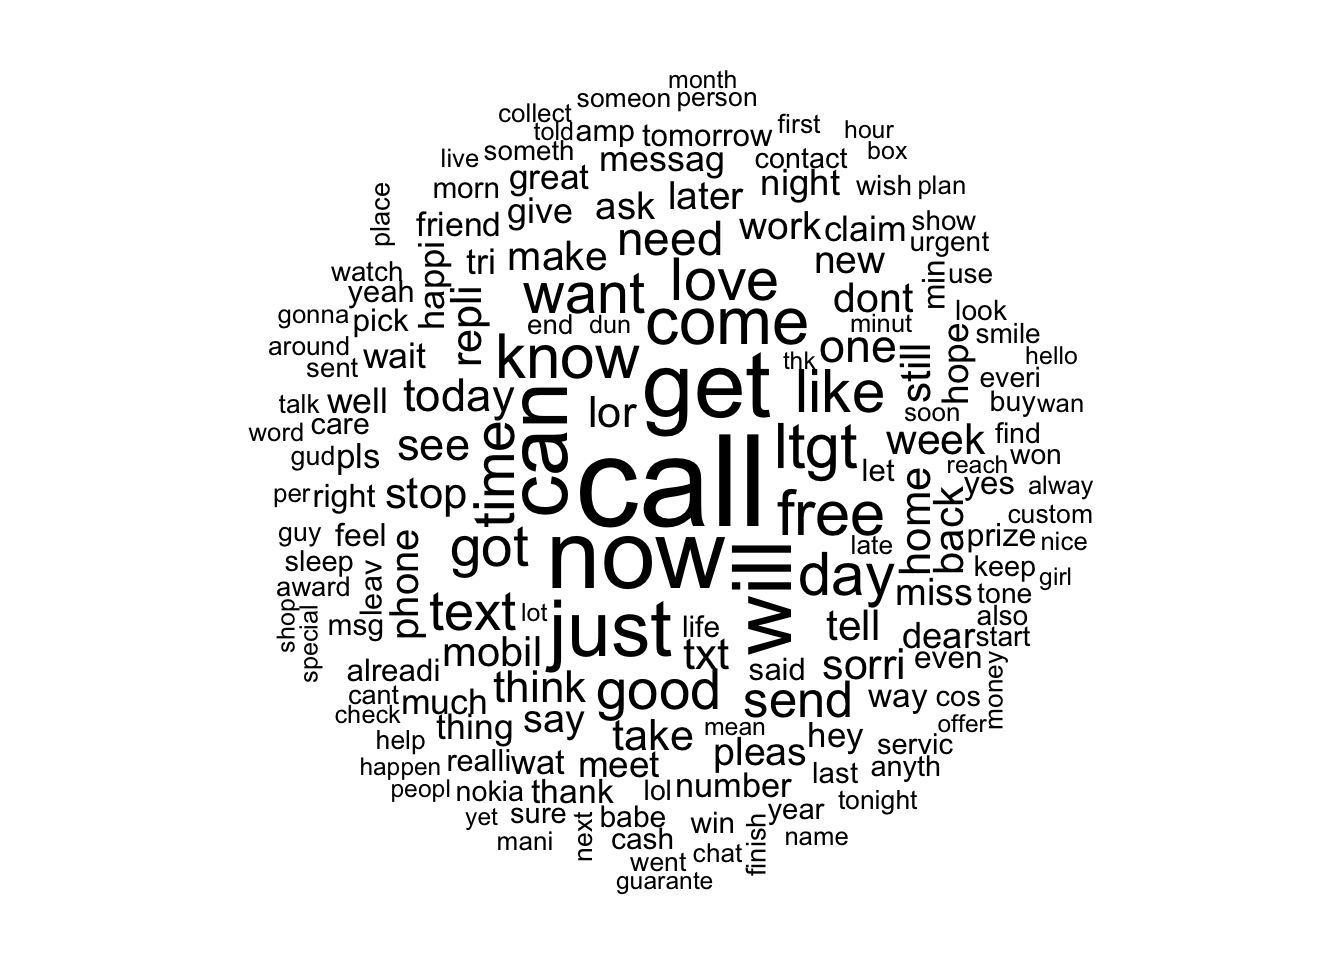
\includegraphics{NaiveBayes_files/figure-latex/unnamed-chunk-21-1.pdf}

\begin{Shaded}
\begin{Highlighting}[]
\KeywordTok{options}\NormalTok{(}\DataTypeTok{warnings=}\DecValTok{2}\NormalTok{) }
\end{Highlighting}
\end{Shaded}

Vemos otras nubes de palabras unas del spam y otra del ham

\begin{Shaded}
\begin{Highlighting}[]
\NormalTok{spam<-}\KeywordTok{subset}\NormalTok{(sms_raw,type}\OperatorTok{==}\StringTok{"spam"}\NormalTok{)}
\NormalTok{ham<-}\KeywordTok{subset}\NormalTok{(sms_raw,type}\OperatorTok{==}\StringTok{"ham"}\NormalTok{)}

\KeywordTok{wordcloud}\NormalTok{(spam}\OperatorTok{$}\NormalTok{text,}\DataTypeTok{max.words =} \DecValTok{40}\NormalTok{,}\DataTypeTok{scale=}\KeywordTok{c}\NormalTok{(}\DecValTok{3}\NormalTok{,}\FloatTok{0.5}\NormalTok{))}
\end{Highlighting}
\end{Shaded}

\begin{verbatim}
## Warning in tm_map.SimpleCorpus(corpus, tm::removePunctuation):
## transformation drops documents
\end{verbatim}

\begin{verbatim}
## Warning in tm_map.SimpleCorpus(corpus, function(x) tm::removeWords(x,
## tm::stopwords())): transformation drops documents
\end{verbatim}

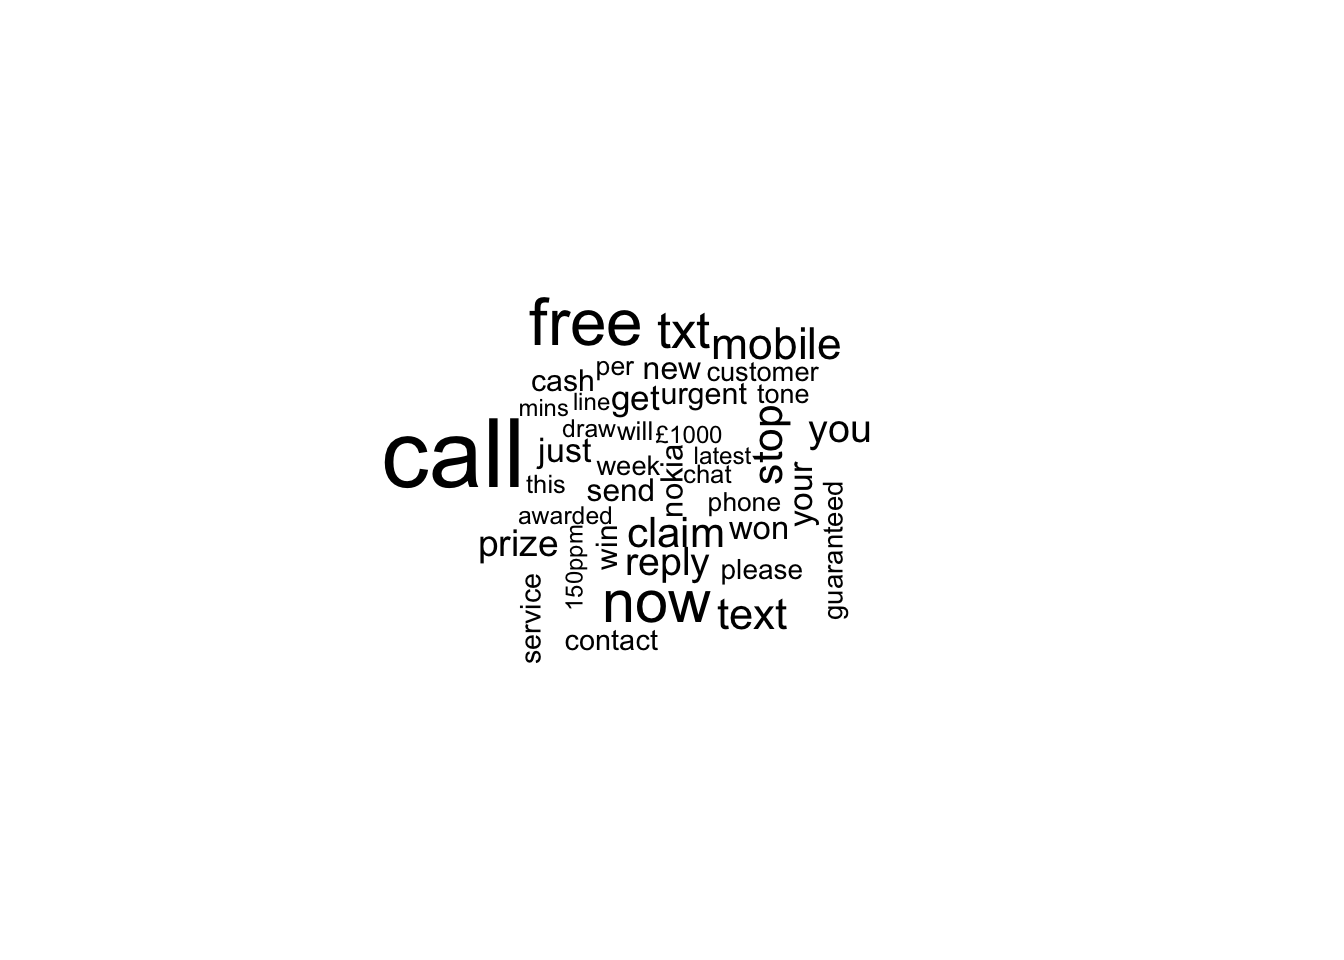
\includegraphics{NaiveBayes_files/figure-latex/unnamed-chunk-22-1.pdf}

\begin{Shaded}
\begin{Highlighting}[]
\KeywordTok{wordcloud}\NormalTok{(ham}\OperatorTok{$}\NormalTok{text,}\DataTypeTok{max.words =} \DecValTok{40}\NormalTok{, }\DataTypeTok{scale=}\KeywordTok{c}\NormalTok{(}\DecValTok{3}\NormalTok{,}\FloatTok{0.5}\NormalTok{))}
\end{Highlighting}
\end{Shaded}

\begin{verbatim}
## Warning in tm_map.SimpleCorpus(corpus, tm::removePunctuation):
## transformation drops documents

## Warning in tm_map.SimpleCorpus(corpus, tm::removePunctuation):
## transformation drops documents
\end{verbatim}

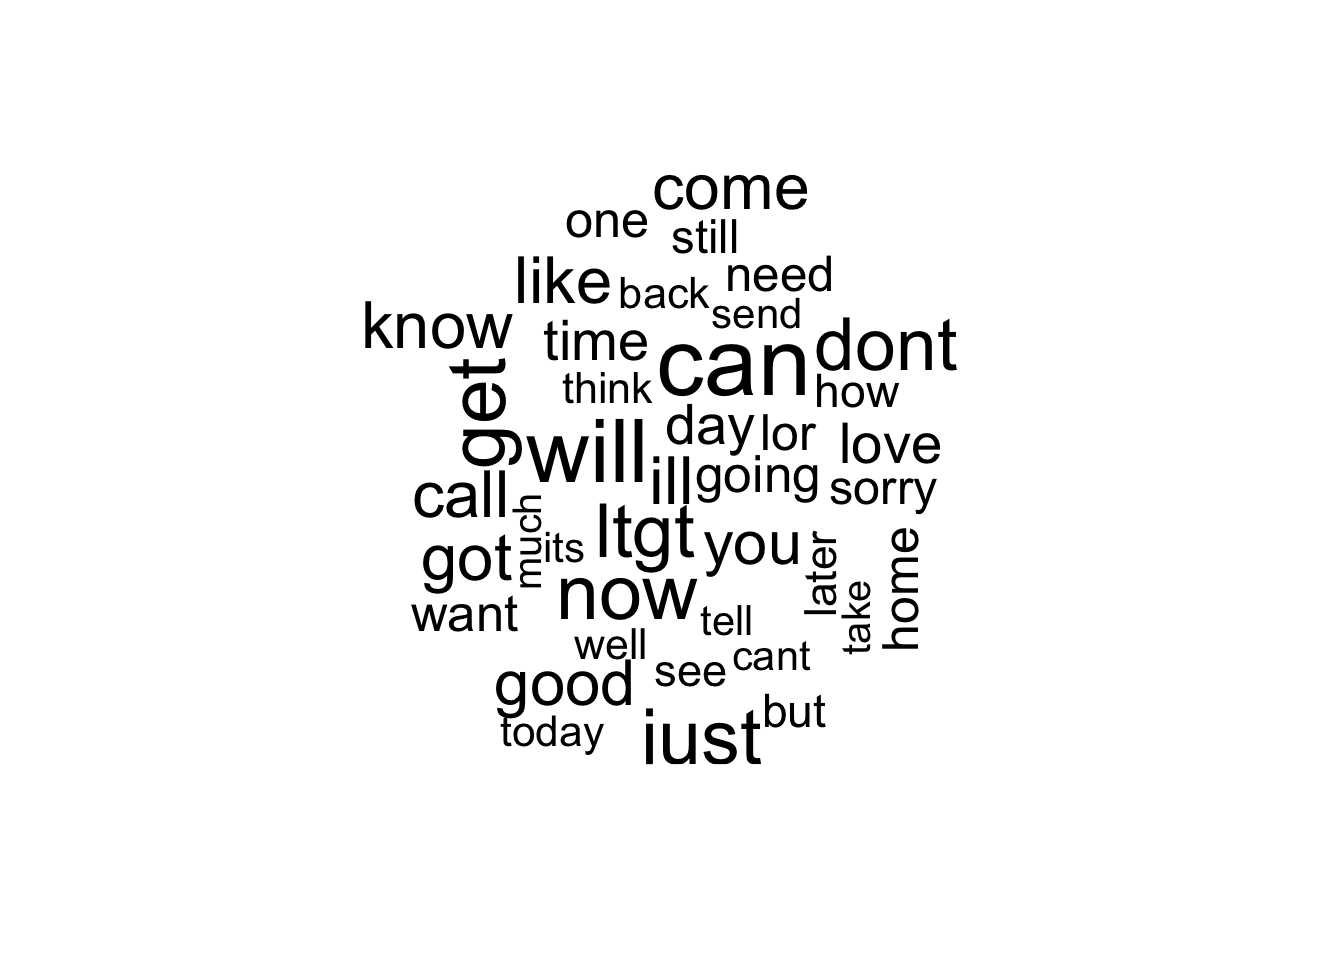
\includegraphics{NaiveBayes_files/figure-latex/unnamed-chunk-22-2.pdf}

Vamos hacer más limpio la prueba, haciendo que solo busque la que tenga
más de 5 menciones

\begin{Shaded}
\begin{Highlighting}[]
\KeywordTok{findFreqTerms}\NormalTok{(sms_dtm_train,}\DecValTok{5}\NormalTok{)}
\end{Highlighting}
\end{Shaded}

\begin{verbatim}
##    [1] "£wk"           "abiola"        "abl"           "abt"          
##    [5] "accept"        "access"        "account"       "across"       
##    [9] "activ"         "actual"        "add"           "address"      
##   [13] "admir"         "adult"         "advanc"        "aft"          
##   [17] "afternoon"     "aftr"          "age"           "ago"          
##   [21] "ahead"         "aight"         "aint"          "air"          
##   [25] "aiyah"         "alex"          "almost"        "alon"         
##   [29] "alreadi"       "alright"       "alrit"         "also"         
##   [33] "alway"         "amp"           "angri"         "announc"      
##   [37] "anoth"         "answer"        "anybodi"       "anymor"       
##   [41] "anyon"         "anyth"         "anytim"        "anyway"       
##   [45] "apart"         "app"           "appli"         "appoint"      
##   [49] "appreci"       "april"         "ard"           "area"         
##   [53] "argument"      "arm"           "around"        "arrang"       
##   [57] "arrest"        "arriv"         "asap"          "ask"          
##   [61] "askd"          "asleep"        "ass"           "attempt"      
##   [65] "auction"       "avail"         "ave"           "avoid"        
##   [69] "await"         "award"         "away"          "awesom"       
##   [73] "babe"          "babi"          "back"          "bad"          
##   [77] "bag"           "bak"           "balanc"        "bank"         
##   [81] "bare"          "bath"          "batteri"       "bcoz"         
##   [85] "bcum"          "bday"          "beauti"        "becom"        
##   [89] "bed"           "bedroom"       "begin"         "believ"       
##   [93] "belli"         "best"          "better"        "bid"          
##   [97] "big"           "bill"          "bird"          "birthday"     
##  [101] "bit"           "black"         "blank"         "bless"        
##  [105] "blue"          "bluetooth"     "bodi"          "bold"         
##  [109] "bonus"         "boo"           "book"          "bore"         
##  [113] "boss"          "bother"        "bout"          "bowl"         
##  [117] "box"           "boy"           "boytoy"        "brand"        
##  [121] "break"         "breath"        "brilliant"     "bring"        
##  [125] "brother"       "bslvyl"        "btnationalr"   "budget"       
##  [129] "bugi"          "bus"           "busi"          "buy"          
##  [133] "buzz"          "cabin"         "cafe"          "cal"          
##  [137] "call"          "caller"        "callertun"     "camcord"      
##  [141] "came"          "camera"        "can"           "cancel"       
##  [145] "cant"          "car"           "card"          "care"         
##  [149] "carlo"         "case"          "cash"          "cashbal"      
##  [153] "catch"         "caus"          "chanc"         "chang"        
##  [157] "charact"       "charg"         "chariti"       "chat"         
##  [161] "cheap"         "check"         "cheer"         "chennai"      
##  [165] "chikku"        "childish"      "children"      "chines"       
##  [169] "choic"         "choos"         "christma"      "cine"         
##  [173] "cinema"        "claim"         "class"         "clean"        
##  [177] "clear"         "click"         "clock"         "close"        
##  [181] "club"          "code"          "coffe"         "coin"         
##  [185] "cold"          "colleagu"      "collect"       "colleg"       
##  [189] "colour"        "come"          "comin"         "comp"         
##  [193] "compani"       "competit"      "complet"       "complimentari"
##  [197] "comput"        "concentr"      "condit"        "confid"       
##  [201] "confirm"       "congrat"       "congratul"     "connect"      
##  [205] "contact"       "content"       "convey"        "cook"         
##  [209] "cool"          "copi"          "correct"       "cos"          
##  [213] "cost"          "countri"       "coupl"         "cours"        
##  [217] "cover"         "coz"           "crave"         "crazi"        
##  [221] "credit"        "cri"           "croydon"       "cuddl"        
##  [225] "cum"           "cup"           "current"       "custcar"      
##  [229] "custom"        "cut"           "cute"          "cuz"          
##  [233] "dad"           "daddi"         "damn"          "darl"         
##  [237] "darlin"        "darren"        "dat"           "date"         
##  [241] "day"           "dead"          "deal"          "dear"         
##  [245] "decid"         "deep"          "definit"       "del"          
##  [249] "delet"         "deliv"         "deliveri"      "den"          
##  [253] "depend"        "detail"        "dey"           "didnt"        
##  [257] "die"           "differ"        "difficult"     "digit"        
##  [261] "din"           "dinner"        "direct"        "dis"          
##  [265] "discount"      "discuss"       "disturb"       "dnt"          
##  [269] "doctor"        "doesnt"        "dog"           "doin"         
##  [273] "dollar"        "don"           "don‘t"         "done"         
##  [277] "dont"          "door"          "doubl"         "download"     
##  [281] "draw"          "dream"         "drink"         "drive"        
##  [285] "drop"          "drug"          "dude"          "dun"          
##  [289] "dunno"         "dvd"           "earli"         "earlier"      
##  [293] "easi"          "eat"           "eatin"         "either"       
##  [297] "els"           "email"         "embarass"      "empti"        
##  [301] "end"           "enemi"         "energi"        "england"      
##  [305] "enjoy"         "enough"        "enter"         "entri"        
##  [309] "envelop"       "especi"        "etc"           "euro"         
##  [313] "eve"           "even"          "ever"          "everi"        
##  [317] "everyon"       "everyth"       "exact"         "exam"         
##  [321] "excel"         "excit"         "excus"         "expect"       
##  [325] "experi"        "expir"         "extra"         "eye"          
##  [329] "face"          "facebook"      "fact"          "fall"         
##  [333] "famili"        "fanci"         "fantasi"       "fantast"      
##  [337] "far"           "fast"          "fat"           "father"       
##  [341] "fault"         "feel"          "felt"          "fetch"        
##  [345] "fight"         "figur"         "file"          "fill"         
##  [349] "film"          "final"         "find"          "fine"         
##  [353] "finger"        "finish"        "first"         "five"         
##  [357] "fix"           "flight"        "flirt"         "flower"       
##  [361] "follow"        "fone"          "food"          "forev"        
##  [365] "forget"        "forgot"        "forward"       "found"        
##  [369] "free"          "freemsg"       "freephon"      "fren"         
##  [373] "fri"           "friday"        "friend"        "friendship"   
##  [377] "frm"           "frnd"          "frnds"         "fuck"         
##  [381] "full"          "fullonsmscom"  "fun"           "funni"        
##  [385] "futur"         "gal"           "game"          "gap"          
##  [389] "gas"           "gave"          "gay"           "gentl"        
##  [393] "get"           "gettin"        "gift"          "girl"         
##  [397] "give"          "glad"          "god"           "goe"          
##  [401] "goin"          "gone"          "gonna"         "good"         
##  [405] "goodmorn"      "goodnight"     "got"           "goto"         
##  [409] "gotta"         "great"         "green"         "greet"        
##  [413] "grin"          "group"         "guarante"      "gud"          
##  [417] "guess"         "guy"           "gym"           "haf"          
##  [421] "haha"          "hai"           "hair"          "half"         
##  [425] "hand"          "hang"          "happen"        "happi"        
##  [429] "hard"          "hav"           "havent"        "head"         
##  [433] "hear"          "heard"         "heart"         "heavi"        
##  [437] "hee"           "hell"          "hello"         "help"         
##  [441] "hey"           "hgsuiteland"   "high"          "hit"          
##  [445] "hiya"          "hmm"           "hmmm"          "hmv"          
##  [449] "hol"           "hold"          "holder"        "holiday"      
##  [453] "home"          "honey"         "hook"          "hop"          
##  [457] "hope"          "horni"         "hospit"        "hot"          
##  [461] "hotel"         "hour"          "hous"          "housemaid"    
##  [465] "how"           "howev"         "howz"          "hrs"          
##  [469] "hug"           "huh"           "hungri"        "hurri"        
##  [473] "hurt"          "iam"           "ice"           "idea"         
##  [477] "identifi"      "ignor"         "ill"           "imagin"       
##  [481] "imma"          "immedi"        "import"        "inc"          
##  [485] "inch"          "includ"        "india"         "indian"       
##  [489] "info"          "inform"        "instead"       "interest"     
##  [493] "interview"     "invit"         "ipod"          "irrit"        
##  [497] "ish"           "issu"          "ive"           "izzit"        
##  [501] "januari"       "jay"           "job"           "john"         
##  [505] "join"          "joke"          "joy"           "jus"          
##  [509] "just"          "juz"           "kalli"         "kate"         
##  [513] "keep"          "kept"          "key"           "kick"         
##  [517] "kid"           "kill"          "kind"          "kinda"        
##  [521] "king"          "kiss"          "knew"          "know"         
##  [525] "knw"           "ladi"          "land"          "landlin"      
##  [529] "laptop"        "lar"           "last"          "late"         
##  [533] "later"         "latest"        "laugh"         "lazi"         
##  [537] "ldn"           "lead"          "learn"         "least"        
##  [541] "leav"          "lect"          "left"          "leh"          
##  [545] "lei"           "lemm"          "less"          "lesson"       
##  [549] "let"           "letter"        "liao"          "librari"      
##  [553] "lick"          "lie"           "life"          "lift"         
##  [557] "light"         "like"          "line"          "link"         
##  [561] "list"          "listen"        "littl"         "live"         
##  [565] "load"          "loan"          "local"         "locat"        
##  [569] "log"           "login"         "lol"           "long"         
##  [573] "longer"        "look"          "lor"           "lose"         
##  [577] "lost"          "lot"           "lovabl"        "love"         
##  [581] "lover"         "loverboy"      "loyalti"       "ltd"          
##  [585] "ltdecimalgt"   "ltgt"          "lttimegt"      "luck"         
##  [589] "lucki"         "lunch"         "luv"           "made"         
##  [593] "mah"           "mail"          "make"          "man"          
##  [597] "mani"          "march"         "mark"          "marri"        
##  [601] "marriag"       "match"         "mate"          "matter"       
##  [605] "maxim"         "may"           "mayb"          "mean"         
##  [609] "meant"         "med"           "medic"         "meet"         
##  [613] "meh"           "mell"          "member"        "men"          
##  [617] "menu"          "merri"         "messag"        "met"          
##  [621] "mid"           "midnight"      "might"         "min"          
##  [625] "mind"          "mine"          "minut"         "miracl"       
##  [629] "miss"          "mistak"        "moan"          "mob"          
##  [633] "mobil"         "mobileupd"     "mode"          "mom"          
##  [637] "moment"        "mon"           "monday"        "money"        
##  [641] "month"         "mood"          "moon"          "morn"         
##  [645] "motorola"      "move"          "movi"          "mrng"         
##  [649] "mrt"           "msg"           "msgs"          "mths"         
##  [653] "much"          "mum"           "murder"        "music"        
##  [657] "must"          "muz"           "nah"           "nake"         
##  [661] "name"          "nation"        "natur"         "naughti"      
##  [665] "near"          "need"          "net"           "network"      
##  [669] "neva"          "never"         "new"           "news"         
##  [673] "next"          "nice"          "nigeria"       "night"        
##  [677] "nite"          "nobodi"        "noe"           "nokia"        
##  [681] "none"          "noon"          "nope"          "normal"       
##  [685] "noth"          "notic"         "now"           "ntt"          
##  [689] "num"           "number"        "nxt"           "nyt"          
##  [693] "offer"         "offic"         "offici"        "okay"         
##  [697] "oki"           "old"           "omw"           "one"          
##  [701] "onlin"         "oop"           "open"          "oper"         
##  [705] "opinion"       "opt"           "optout"        "orang"        
##  [709] "orchard"       "order"         "oredi"         "oso"          
##  [713] "other"         "otherwis"      "outsid"        "pack"         
##  [717] "page"          "paid"          "pain"          "paper"        
##  [721] "parent"        "park"          "part"          "parti"        
##  [725] "partner"       "pass"          "passion"       "password"     
##  [729] "past"          "pay"           "peac"          "peopl"        
##  [733] "per"           "person"        "pete"          "phone"        
##  [737] "photo"         "pic"           "pick"          "pictur"       
##  [741] "piec"          "pix"           "pizza"         "place"        
##  [745] "plan"          "plane"         "play"          "player"       
##  [749] "pleas"         "pleasur"       "pls"           "plus"         
##  [753] "plz"           "pmin"          "pmsg"          "pobox"        
##  [757] "poboxwwq"      "point"         "poli"          "polic"        
##  [761] "poor"          "pop"           "possibl"       "post"         
##  [765] "pound"         "power"         "pple"          "ppm"          
##  [769] "practic"       "pray"          "prefer"        "prepar"       
##  [773] "press"         "pretti"        "price"         "princess"     
##  [777] "privat"        "prize"         "prob"          "probabl"      
##  [781] "problem"       "process"       "project"       "promis"       
##  [785] "pub"           "put"           "qualiti"       "question"     
##  [789] "quick"         "quit"          "quiz"          "quot"         
##  [793] "rain"          "rate"          "rather"        "rcvd"         
##  [797] "reach"         "read"          "readi"         "real"         
##  [801] "realiz"        "realli"        "reason"        "receipt"      
##  [805] "receiv"        "recent"        "record"        "refer"        
##  [809] "regard"        "regist"        "remain"        "rememb"       
##  [813] "remind"        "remov"         "rent"          "rental"       
##  [817] "repli"         "repres"        "request"       "respond"      
##  [821] "respons"       "rest"          "result"        "return"       
##  [825] "reveal"        "review"        "right"         "ring"         
##  [829] "rington"       "rite"          "road"          "rock"         
##  [833] "room"          "roommat"       "rose"          "round"        
##  [837] "rowwjhl"       "rpli"          "rreveal"       "run"          
##  [841] "sad"           "sae"           "safe"          "said"         
##  [845] "sale"          "sam"           "sat"           "saturday"     
##  [849] "savamob"       "save"          "saw"           "say"          
##  [853] "sch"           "school"        "score"         "scream"       
##  [857] "sea"           "search"        "season"        "sec"          
##  [861] "second"        "secret"        "see"           "seem"         
##  [865] "seen"          "select"        "self"          "sell"         
##  [869] "semest"        "send"          "sens"          "sent"         
##  [873] "serious"       "servic"        "set"           "settl"        
##  [877] "sex"           "sexi"          "shall"         "share"        
##  [881] "shd"           "ship"          "shirt"         "shit"         
##  [885] "shop"          "short"         "show"          "shower"       
##  [889] "shuhui"        "sick"          "side"          "sigh"         
##  [893] "sight"         "sign"          "silent"        "simpl"        
##  [897] "sinc"          "sing"          "singl"         "sir"          
##  [901] "sis"           "sister"        "sit"           "situat"       
##  [905] "sky"           "slave"         "sleep"         "slept"        
##  [909] "slow"          "slowli"        "small"         "smile"        
##  [913] "smoke"         "sms"           "smth"          "snow"         
##  [917] "sofa"          "solv"          "somebodi"      "someon"       
##  [921] "someth"        "sometim"       "somewher"      "song"         
##  [925] "soni"          "sonyericsson"  "soon"          "sorri"        
##  [929] "sort"          "sound"         "space"         "speak"        
##  [933] "special"       "specialcal"    "spend"         "spent"        
##  [937] "spoke"         "sport"         "spree"         "stand"        
##  [941] "star"          "start"         "statement"     "station"      
##  [945] "stay"          "std"           "still"         "stock"        
##  [949] "stop"          "store"         "stori"         "str"          
##  [953] "straight"      "street"        "strong"        "student"      
##  [957] "studi"         "stuff"         "stupid"        "style"        
##  [961] "sub"           "subscrib"      "success"       "summer"       
##  [965] "sun"           "sunday"        "sunshin"       "support"      
##  [969] "suppos"        "sure"          "surpris"       "sweet"        
##  [973] "swing"         "system"        "take"          "talk"         
##  [977] "tampa"         "tcs"           "teach"         "team"         
##  [981] "tear"          "teas"          "tel"           "tell"         
##  [985] "ten"           "tenerif"       "term"          "test"         
##  [989] "text"          "thank"         "thanx"         "that"         
##  [993] "thing"         "think"         "thinkin"       "thk"          
##  [997] "thnk"          "tho"           "though"        "thought"      
## [1001] "throw"         "thru"          "tht"           "thur"         
## [1005] "ticket"        "til"           "till"          "time"         
## [1009] "tire"          "titl"          "tmr"           "tncs"         
## [1013] "today"         "togeth"        "told"          "tomo"         
## [1017] "tomorrow"      "tone"          "tonight"       "tonit"        
## [1021] "took"          "top"           "tot"           "total"        
## [1025] "touch"         "tough"         "tour"          "toward"       
## [1029] "town"          "track"         "train"         "transact"     
## [1033] "treat"         "tri"           "trip"          "troubl"       
## [1037] "true"          "trust"         "truth"         "tscs"         
## [1041] "ttyl"          "tuesday"       "turn"          "twice"        
## [1045] "two"           "txt"           "txting"        "txts"         
## [1049] "type"          "ufind"         "ugh"           "umma"         
## [1053] "uncl"          "understand"    "unless"        "unlimit"      
## [1057] "unredeem"      "unsub"         "unsubscrib"    "updat"        
## [1061] "ure"           "urgent"        "urself"        "use"          
## [1065] "usf"           "usual"         "uve"           "valentin"     
## [1069] "valid"         "valu"          "vari"          "verifi"       
## [1073] "via"           "video"         "visit"         "voic"         
## [1077] "voucher"       "wait"          "wake"          "walk"         
## [1081] "wan"           "wana"          "wanna"         "want"         
## [1085] "wap"           "warm"          "wast"          "wat"          
## [1089] "watch"         "water"         "way"           "weak"         
## [1093] "wear"          "weather"       "wed"           "wednesday"    
## [1097] "weed"          "week"          "weekend"       "weight"       
## [1101] "welcom"        "well"          "wen"           "went"         
## [1105] "wer"           "wet"           "what"          "whatev"       
## [1109] "whenev"        "whole"         "wid"           "wif"          
## [1113] "wife"          "wil"           "will"          "win"          
## [1117] "wine"          "winner"        "wish"          "wit"          
## [1121] "within"        "without"       "wiv"           "wkli"         
## [1125] "wnt"           "woke"          "won"           "wonder"       
## [1129] "wont"          "word"          "work"          "workin"       
## [1133] "world"         "worri"         "worth"         "wot"          
## [1137] "wow"           "write"         "wrong"         "wun"          
## [1141] "wwwgetzedcouk" "xmas"          "xxx"           "yahoo"        
## [1145] "yar"           "yeah"          "year"          "yep"          
## [1149] "yes"           "yest"          "yesterday"     "yet"          
## [1153] "yoga"          "yogasana"      "yrs"           "yun"          
## [1157] "yup"
\end{verbatim}

\begin{Shaded}
\begin{Highlighting}[]
\NormalTok{sms_freq_words<-}\KeywordTok{findFreqTerms}\NormalTok{(sms_dtm_train,}\DecValTok{5}\NormalTok{)}

\KeywordTok{str}\NormalTok{(sms_freq_words)}
\end{Highlighting}
\end{Shaded}

\begin{verbatim}
##  chr [1:1157] "£wk" "abiola" "abl" "abt" "accept" "access" "account" ...
\end{verbatim}

\begin{Shaded}
\begin{Highlighting}[]
\NormalTok{sms_dtm_freq_train<-}\StringTok{ }\NormalTok{sms_dtm_train[ , sms_freq_words]}
\NormalTok{sms_dtm_freq_test <-}\StringTok{ }\NormalTok{sms_dtm_test[ , sms_freq_words]         }


\NormalTok{##hacer una funcion que nos diga si es spam o no}

\NormalTok{convert_counts <-}\StringTok{ }\ControlFlowTok{function}\NormalTok{(x) \{}
\NormalTok{    x <-}\StringTok{ }\KeywordTok{ifelse}\NormalTok{(x }\OperatorTok{>}\StringTok{ }\DecValTok{0}\NormalTok{, }\StringTok{"Yes"}\NormalTok{, }\StringTok{"No"}\NormalTok{)}
\NormalTok{\}}


\NormalTok{sms_train <-}\StringTok{ }\KeywordTok{apply}\NormalTok{(sms_dtm_freq_train, }\DataTypeTok{MARGIN =} \DecValTok{2}\NormalTok{,}
\NormalTok{                                       convert_counts)}
\NormalTok{sms_test <-}\StringTok{ }\KeywordTok{apply}\NormalTok{(sms_dtm_freq_test, }\DataTypeTok{MARGIN =} \DecValTok{2}\NormalTok{,}
\NormalTok{                                      convert_counts)}

\KeywordTok{str}\NormalTok{(sms_train)}
\end{Highlighting}
\end{Shaded}

\begin{verbatim}
##  chr [1:4169, 1:1157] "No" "No" "No" "No" "No" "No" "No" "No" "No" ...
##  - attr(*, "dimnames")=List of 2
##   ..$ Docs : chr [1:4169] "1" "2" "3" "4" ...
##   ..$ Terms: chr [1:1157] "£wk" "abiola" "abl" "abt" ...
\end{verbatim}

\begin{Shaded}
\begin{Highlighting}[]
\KeywordTok{str}\NormalTok{(sms_test)}
\end{Highlighting}
\end{Shaded}

\begin{verbatim}
##  chr [1:1390, 1:1157] "No" "No" "No" "No" "No" "No" "No" "No" "No" ...
##  - attr(*, "dimnames")=List of 2
##   ..$ Docs : chr [1:1390] "4170" "4171" "4172" "4173" ...
##   ..$ Terms: chr [1:1157] "£wk" "abiola" "abl" "abt" ...
\end{verbatim}

\subsection{Haciendo el modelo y
evaluando}\label{haciendo-el-modelo-y-evaluando}

\begin{Shaded}
\begin{Highlighting}[]
\KeywordTok{install.packages}\NormalTok{(}\StringTok{"e1071"}\NormalTok{,}\DataTypeTok{repos =} \StringTok{"http://cran.us.r-project.org"}\NormalTok{)}
\end{Highlighting}
\end{Shaded}

\begin{verbatim}
## 
##   There is a binary version available but the source version is
##   later:
##       binary  source needs_compilation
## e1071  1.7-0 1.7-0.1              TRUE
\end{verbatim}

\begin{verbatim}
## installing the source package 'e1071'
\end{verbatim}

\begin{Shaded}
\begin{Highlighting}[]
\KeywordTok{library}\NormalTok{(e1071)}
\end{Highlighting}
\end{Shaded}

\begin{Shaded}
\begin{Highlighting}[]
\NormalTok{sms_classifier <-}\StringTok{ }\KeywordTok{naiveBayes}\NormalTok{(sms_train, sms_train_labels)}

\CommentTok{#making predictions}
\NormalTok{sms_test_pred <-}\StringTok{ }\KeywordTok{predict}\NormalTok{(sms_classifier, sms_test)}

\KeywordTok{head}\NormalTok{(sms_test_pred)}
\end{Highlighting}
\end{Shaded}

\begin{verbatim}
## factor(0)
## Levels:
\end{verbatim}

\begin{Shaded}
\begin{Highlighting}[]
\CommentTok{#install.packages("gmodels", repos = "http://cran.us.r-project.org")}
\CommentTok{#library(gmodels)}

\KeywordTok{length}\NormalTok{(sms_test_pred)}
\end{Highlighting}
\end{Shaded}

\begin{verbatim}
## [1] 0
\end{verbatim}

\begin{Shaded}
\begin{Highlighting}[]
\CommentTok{#CrossTable(sms_test_pred, sms_test_labels,}
 \CommentTok{#   prop.chisq = FALSE, prop.t = FALSE,}
  \CommentTok{#  dnn = c('predicted', 'actual'))}

\CommentTok{#table(sms_test_pred,sms_test_labels)}
\end{Highlighting}
\end{Shaded}

\subsection{Buscando mejorar usando el estimador
laplace}\label{buscando-mejorar-usando-el-estimador-laplace}

\begin{Shaded}
\begin{Highlighting}[]
\NormalTok{sms_classifier2<-}\KeywordTok{naiveBayes}\NormalTok{(sms_train,sms_train_labels,}\DataTypeTok{laplace =} \DecValTok{1}\NormalTok{)}
\NormalTok{sms_tes_pred2<-}\KeywordTok{predict}\NormalTok{(sms_classifier2,sms_test)}

\CommentTok{#CrossTable(sms_tes_pred2,sms_test_labels,prop.chisq = FALSE, prop.t = FALSE,}
         \CommentTok{#  dnn = c("predicted","actual"))}

\CommentTok{#table(sms_tes_pred2,sms_test_labels)}
\end{Highlighting}
\end{Shaded}


\end{document}
